\chapter{Εισαγωγή}

Σε αυτή την εργασία θα εξερευνήσουμε κάποια λογικά κυκλωματικά στοιχεία που μπορούν να χρησιμοποιηθούν για την κατασκευή μιας απλής Αριθμητικής
Λογικής Μονάδας. Αρχικά θα γίνει μια ανάλυση της αρχικής ιδέας του περίφημου θεωρητικού φυσικού και δασκάλου, Richard P. Feynman
για την θεωρητική προσέγγιση ενός υπολογιστή που θα χρησιμοποιεί του κβαντικούς νόμους της φυσής για να τελεί έργο των ανθρώπων.

Έπειτα, θα μιλήσουμε σε έκταση για μερικά βασικά θεμέλια της κλασικής όσο και της κβαντικής θεωρίας της Υπολογιστικής που θα χρειαστούν για την
κατανόηση της εργασίας. Στο δεύτερο κεφάλαιο θα γίνει μια βιβλιογραφική ανασκόπηση του πεδίου της Κβαντικής Υπολογιστικής και Λογικής Σχεδίασης
με σκοπό ο αναγνώστης να αποκτήσει ένα ολοκληρωμένο πλαίσιο για την βαθύτερη κατανόηση της εργασίας.

Μετά την βιβλιογραφική ανασκόπηση ακολουθούν τα κυριώς κεφάλαια της εργασίας. Τα κύρια κεφάλαια έχουν χωριστεί σε δυο μερη: το πρώτο μέρος αναλύει
την υλοποίηση των κβαντικών λογικών κυκλωμάτων χρησιμοποιώντας την γλώσσα προγραμματισμού Python και του Qiskit, ένα Σετ Ανάπτυξης Λογισμικού
(Software Development Kit) και στο δεύτερο μέρος θα αναλυθεί η αρχιτεκτονική συνόλου εντολών της μονάδας καταλήγοντας με την σύνθεση όλων το προαναφερόμενων κυκλωμάτων σε μια συνδυαστική μονάδα.

Το επόμενο κεφάλαιο, αναγράφει τα αποτελέσματα των προσωμειώσεων χρησιμοποιώντας τον προσωμοιοτή Aer της IBM για τα κβαντικά κυκλώματα καθώς
και τα αποτελέσματα και τις μετρήσεις από των κβαντικό υπολογιστή της IBM, τον System One.

Τέλος, τα τελευταία δυο κεφάλαια της εργασίας θα χρησιμοποιηθούν για τον σχολιασμό της εργασίας, το πώς μπορεί η εργασία να βελτιωθεί καθώς
και μια απλή καταγραφή των συμπερασμάτων μας.

\section{"Κβαντομηχανικοί Υπολογιστές"}
Το 1984, ο περίφημος θεωρητικός και νομπελίστας φυσικός Richard P. Feynman έδωσε μια ομιλία κατά την οποία προσπάθησε να
εκφράσει αναλυτικά τα φυσικά όρια των υπολογιστών της εποχής λόγω των νόμων της Φυσικής δίνοντας παραδείγματα προήγουμενων εργασίων του Bennett,
Fredkin και Toffoli.
Λέει ο Feynman \cite{Feynman1986} ότι συζητώντας με τον Bennett για το άν υπάρχουν θεμελιώδη όρια στους υπολογιστές λόγω των κβαντομηχανικών νόμων
και της αρχής της απροσδιοριστίας, πως δεν υπάρχει όριο στο πόσο μικρά μπορούμε να φτιάξουμε τα επιμέρους κομμάτια ενός υπολογιστή. Σημειώνει όμως
ότι οι υπολογίστες τέτοιου μεγέθους πρέπει να υπακούν στην αρχή της αντιστρεψιμότητας των κβαντομηχανικών νόμων στο χρόνο.
Ένα άλλο πρόβλημα που συζητά ο Feynman είναι το πρόβλημα των απωλειών σε θερμότητα των υπολογιστών λόγω της μη-αντιστρέψιμης λειτουργείας τους.
Το θεωρητικό πλαίσιο που μιλά για το πόσο ελάχιστο πόσο ενέργειας απόβάλλει ένα σύστημα για την εκτέλεση μιας στοιχειώδους, μη-αναστρέψιμης λογικής πράξης είναι:

\begin{equation}
    E = k_y T \ln 2 \approx 10^{-21} Joule
\end{equation}

Σύμφωνα με τον Μαρμόρκο \cite{Marmorkos2024} η σχέση ονομάζεται σχέση Shannon-von Neumann-Landauer (SNL), η θερμοκρασία $T$ είναι ίση με την
θερμοκρασία δωματίου σε βαθμούς Kelvin ($T = 300 K$) και $k_y$ είναι η σταθερά του Boltzmann ($k_y = 1.380649 \times 10^{-23}J \cdot K^{-1}$).
Καταλαβαίνουμε από την παραπάνω σχέση ότι όσο περισσότερα μη-αναστρέψιμα λογικά στοιχεία έχει ένα υπολογιστικό σύστημα τόσο μεγαλύτερη απώλεια
θα έχει. Επίσης αναφέρει ότι αν θα θέλαμε να κατασκευάσουμε ένα τέτοιο υπολογιστή, το σύστημα θα χρειαζόταν περίπου $3kW$
ενέργειας για την λειτουργία του - ισοδύναμη με την αναγκή ενέργειας 1000 κατοίκων μιας πόλης!

Ο Feynman \cite{Feynman1986} αναφέρει πως θα μπορούσαμε να αποφύγουμε την τεράστια σπατάλη ενέργειας χρησιμοποιώντας επαγωγικά στοιχεία για την αποθήκευση τής αλλά ακομά και οι μοντέρνες τεχνικές λιθογραφίας για την παραγωγή επεξεργαστών υπολογιστών δεν μπορεί να το καταφέρει για την 
μαζική παραγωγή τέτοιων εξαρτημάτων. Για τον λόγο αυτό, ο Feynman εξασκεί την ιδέα της χρήσης ατομών (και γενικά κβαντικών συστημάτων όπως
φωτόνια, ηλεκτρόνια κ.ο.κ.) και αντιστρέψιμων λογικών στοιχείων για την τέλεση υπολογισμών. Στο υποκεφάλαιο 1.3 θα μιλήσουμε για τα στοιχεία που
αναλύει και ο Feynman.

\section{Στοιχεία της κλασικής υπολογιστικής}

Πριν προχωρήσουμε στα κβαντομηχανικά θέματα της θεωρίας, θα θέλαμε να κάνουμε μια ανασκοπική ανάλυση κάποιων πολύ σημαντικών αξιωμάτων και θεωριών
της κλασικής θεώρισης της Υπολογιστικής αρχίζοντας από τα βασικότερα όπως το τί είναι ένα δυαδικός αριθμός καταλείγοντας στο πώς μοντελοποιούμε
τα ψηφικά/δυαδικά λογικά στοιχεία χρησιμοποιώντας το κυκλωματικό μοντέλο.

\subsection{Το δυαδικό σύστημα αρίθμησης}

Στην καθημερινότητα μας χρησιμοποιούμε τους αριθμούς για να μπορέσουμε να κάνουμε τις αγορές μας, να υπολογίσουμε εκπτώσεις κ.α. Οι αριθμοί που
χρησιμοποιούν εμείς οι άνθρωποι ονομάζεται δεκαδικό σύστημα αρίθμησης. Στο δεκαδικό (εν συντομία) τα ψηφία που αναπαρηστούν φυσικές ποσότητες είναι
δέκα, τα γνωστά σε όλους μας: $0, 1, 2, 3, 4, 5, 6, 7, 8, 9$. Κάθε δεκαδικός αριθμός μπορεί να αναπαραστήσει οποιαδήποτε μεγάλη πόσοτητα συνδυάζοντας
τα δέκα βασικά δεκαδικά ψηφία (πχ $1947$ μ.Χ. μπορεί να είναι μια χρονική ποσότητα που αναπαριστά ένα έτος μετά από μια κοινή χρονική αρχή). Σύμφωνα
με τον Mano και Cilleti \cite{ManoCilleti2018} κάθε αριθμός μπορεί να αναπαρασταθεί σε κάποιο θεσιακό σύστημα αρίθμησης σύμφωνα με την παρακάτω
σχέση

\begin{equation}
    \sum_{n=0}^{\infty}a_n \times b^n
\end{equation}

όπου $b$ είναι το σύνολο των ψηφίων του θεσιακού συστήματος αναφοράς μας, δηλαδή η βάση του αριθμητικού συστήματος. Στην περίπτωση του δεκαδικού
συστήματος το $b = 10$. Μπορούμε εύκολα να επαληθεύσουμε την παραπάνω σχέση αναλύοντας τον δεκαδικό αριθμό $1947$ σύμφωνα με την σχέση

\begin{equation}
    1947_{10} = 1 \times 10^3 + 9 \times 10^2 + 4 \times 10^1 + 7 \times 10^0
\end{equation}

Όλα τα μοντέρνα υπολογιστικά συστήματα επεξεργάζονται διακριτά στοιχεία και αριθμούς κωδικοποιημένα σε κάποιο θεσιακό σύστημα αρίθμησης. Το πλεον
δημοφιλέστερο σύστημα αριθμήσης για τους υπολογιστές είναι το δυαδικό σύστημα αρίθμησης (binary numeric system). Ο λόγος που χρησιμοποιείται το
δυαδικό σύστημα από οποιοδήποτε άλλο αποδίδεται στο έργο του Shannon \cite{Shannon1940}, όπου αποδεικνυεί ότι τα διακοπτικά κυκλώματα μπορούν 
να μοντελοποιηθούν χρησιμοποιώντας την άλγεβρα Boole, η οποία άλγεβρα χρησιμοποίει δυο τιμές για την τέλεση των πράξεων της. Την άλγεβρα του Boole
την ονομάζουν και άλγεβρα των δυοτιμών οι Mano και Cilleti \cite{ManoCilleti2018}.

Στο δυαδικό σύστημα, το σύνολο των πιθανών τιμών που μπορεί να πάρει ένας αριθμός $a$ είναι δυο

\begin{equation}
    a \in G: \{0, 1\}
\end{equation}

άρα η βάση του σύστηματος είναι $b = 2$. Οι αριθμοί κωδικοποιούνται ως μια ακολουθία από μηδέν ($0$) και ένα ($1$) για την ευκολότερη επεξεργασία
τους από τα λογικά στοιχεία του υπολογιστή. Για παράδειγμα, ο δεκαδικός αριθμός $21_{10}$ μπορεί να γραφεί στο δυαδικό σύστημα αρίθμησης ως εξης

\begin{equation}
    21_{10} = 10101_2 = 1 \times 2^4 + 0 \times 2^3 + 1 \times 2^2 + 0 \times 2^1 + 1 \times 2^0 
\end{equation}

\subsection{Αριθμητική των δυαδικών αριθμών}

Όπως και στο δεκαδικό έτσι και στο δυαδικό σύστημα ισχύουν όλες οι πράξεις - η πρόσθεση, αφαίρεση, ο πολλαπλασιασμός - με κάποιες μικρές
ιδιαιτερότητες τις οποίες θα αναλύσουμε σε αυτό το κεφάλαιο.

Στην πρόσθεση δυαδικών αριθμών υπάρχουν οι εξής κανόνες

\begin{enumerate}
    \item $0 + 0 = 0$
    \item $0 + 1 = 1 + 0 = 1$
    \item $1 + 1 = 10$, όπου το αριστερότερο ψηφίο του αθροίσματος ονομάζεται το \textit{σημαντικότερο ψηφίο} (most significant bit, MSB) και
    το δεξιότερο \textit{λιγότερο σημαντικό ψηφίο} (least significant bit, LSB). Σε αυτή την περίπτωση δημιουργείται υπερχείληση στην πράξη,
    όπου σε αυτή τη περίπτωση, γράφεται ένα μηδενικό δεξιότερη θέση του αθροίσματος και μια μονάδα είναι κρατούμενο για την επόμενη πράξη
\end{enumerate}

Στην αφαίρεση δυαδικών αριθμών υπάρχουν οι εξής κανόνες

\begin{enumerate}
    \item $0 - 0 = 0$
    \item $1 - 0 = 0$
    \item $0 - 1 = 1$
    \item $1 - 1 = 0$
\end{enumerate}

Στον πολλαπλασιασμό υπάρχουν οι εξής κανόνες

\begin{enumerate}
    \item $0 \times 0 = 0$
    \item $1 \times 0 = 0 \times 1 = 0$
    \item $1 \times 1 = 1$
\end{enumerate}

Όπως μπορούμε να δούμε οι δυαδικές πράξεις είναι πολύ πιο απλές από τις πράξεις του δεκαδικού συστήματος
πράγμα το οποίο θα μας βοηθήσει αρκέτα παρακάτω όταν αρχίζουμε να συνθέτουμε τα κλασικά και κβαντικά λογικά 
κυκλώματα που θα τελούν αυτές τις πράξεις.

Ακολουθούν και μερικά απλά παραδείγματα πράξεων με δυαδικούς αριθμούς:

\begin{table}[ht]
    \centering
    \begin{tabular}{ccccc}
         & 1 & 1 &  &  \\
         & 1 & 1 & 1 & 1 \\
        $+$ & 1 & 0 & 1 & 0 \\
        \hline
        1 & 1 & 0 & 0 & 1 \\
    \end{tabular}
    \hspace{1cm}
    $\Longleftrightarrow $
    \hspace{1cm}
    $1111_2 + 1010_2 = 11001_2 = 25_{10}$
    \caption{Παράδειγμα δυαδικής πρόσθεσης: $15 + 10$}
\end{table}

\qquad

\begin{table}[ht]
    \centering
    \begin{tabular}{ccccc}
          & 1 & 1 & 1 & 1 \\
        $-$ & 1 & 0 & 1 & 0 \\
        \hline
          & 0 & 1 & 0 & 1 \\
    \end{tabular}
    \hspace{1cm}
    $\Longleftrightarrow $
    \hspace{1cm}
    $1111_2 - 1010_2 = 101_2 = 5_{10}$
    \caption{Παράδειγμα δυαδικής αφαίρεσης: $15 - 10$}
\end{table}

\qquad

\begin{table}[ht]
    \centering
    \begin{tabular}{ccccccc}
        &&&&1&1&1\\
        $\times$&&&&0&1&0\\
        \hline
        &&&&0&1&0\\
        &&&0&1&0&\\
        $+$&&0&1&0&&\\
        \hline
        &&&1&1&1&0\\
    \end{tabular}
    \hspace{1cm}
    $\Longleftrightarrow $
    \hspace{1cm}
    $111_2 \times 10_2 = 1110_2 = 14_{10}$
    \caption{Παράδειγμα δυαδικού πολλαπλασιασμού: $7 \times 2$}
\end{table}

\subsection{Συμπληρώματα των δυαδικών αριθμών}

Σύμφωνα με τους Mano και Cilleti \cite{ManoCilleti2018} τα συμπληρώματα χρησιμοποιούνται για την κατασκευεί οικονομικότερων κυκλωμάτων γιατί
απλουστεύουν την πράξη της αφαίρεσης και της γενικότερης λειτουργίας των λογικών πυλών. Σε αυτή την εργασία χρησιμοποιήσαμε αυτή τη λογική και για
την κατασκευεί των κβαντικών λογικών κυκλωμάτων. Σε αυτό το υποκεφάλαιο θα κάνουμε μια ουσιαστική αναφορά στα συμπληρώματα των δυαδικών αριθμών.

Υπάρχουν δυο είδη συμπληρωμάτων:

\begin{enumerate}
    \item το συμπλήρωμα ως προς την μειωμένη βάση, αλλιώς και συμπλήρωμα-ως-προς-($b-1$) και
    \item το συμπλήρωμα ως προς την βάση, αλλιώς και συμπλήρωμα-ως-προς-$b$
\end{enumerate}

Στην περίπτωση του δυαδικού συστήματος, τα συμπληρώματα θα είναι ως-προς-δυο (2s-complement) και ως-προς-ένα (1s-complement).

Θα αναφέρουμε το πώς μπορεί κανείς να φέρει έναν δυαδικό αριθμό $x$ στο συμπλήρωμα του ως-προς-ένα. Έστω ένας δυαδικός αριθμός $x$, το
συμπλήρωμα-ως-προς-ένα βρίσκεται από την σχέση

\begin{equation}
    (2^n - 1) - x
\end{equation}
όπου $n$ είναι ο αριθμός των ψηφίων του  δυαδικού αριθμού. Ακολουθούν μερικά παραδείγματα:

\begin{itemize}
    \item το συμπλήρωμα-ως-προς-ένα του $111_2 = 7_{10}$ είναι
    \begin{equation}
        (2^3 - 1) - x = (111_2 - 1) - 111_2 = 110 - 111 = 000
    \end{equation}
    \item το συμπλήρωμα-ως-προς-ένα του $10101_2 = 21_{10}$ είναι
    \begin{equation}
        (2^5 - 1) - x = (11111_2 - 1) - 10101_2 = 11110 - 10101 = 01010
    \end{equation}
\end{itemize}

Βέβαια, για να μην χρειάζεται να ακολουθούμε όλη αυτή τη διαδικασία, οι Mano και Cilleti \cite{ManoCilleti2018} μας σημειώνουν ότι
το συμπλήρωμα οποιουδήποτε δυαδικού αριθμού υπολογίζεται με το να αλλάξουμε όλα τα μηδέν σε ένα και το ανάποδο.

Το συμπλήρωμα ως προς το δυο ενός δυαδικού αριθμού $x$ δίνεται από την σχέση

\begin{equation}
    c(n, x) =
    \begin{cases}
        2^n - x, & \text{αν } x \neq 0\\
        0,& \text{αν } x = 0
    \end{cases}
\end{equation}

Αφού θέσαμε τα θεμέλια για τα συμπληρώματα των δυαδικών αριθμών, πριν περάσουμε στα προσημασμένα δυαδικά μεγέθη θα θέλαμε να σημειώσουμε
μερικές πράγματα σε σχέση με τις πράξεις χρησιμοποιώντας συμπληρώματα και πιο συγκεκριμένα με την πράξη της αφαίρεσης. Σημειώνουν ο Mano και
Cilleti \cite{ManoCilleti2018} ότι η αφαίρεση που μαθαίνουμε από το σχολείο περιέχει την έννοια του δανειακού ψηφίου. Δανειακό ψηφίο ονομάζουμε
το ψηφίο που \say{δανειζόμαστε} όταν προσπαθήσουμε να αφαιρέσουμε ένα ψηφίο μικρότερης τάξης από ένα ψηφίο μεγαλύτερης τάξης. Αυτή η μέθοδος
είναι εύλογη και εύκολη στον γραπτό λόγο αλλά όταν θέλουμε να γίνεται μέσω ψηφιακών κυκλωμάτων, αυτή η μέθοδος καταστάται λιγότερο χρήσιμη.
Γι' αυτούς τους λόγους τα ψηφιακά κυκλώματα χρησιμοποιούν την αριθμητική με τα συμπληρώματα για να τελέσουν την αφαίρεση.

Θα θέλαμε να προσθέσουμε ότι οι κανόνες τις αριθμητικής, όπως τους αναλύσαμε στο υπό-κεφάλαιο 1.2.2, δεν αλλάζουν για την τέλεση της πρόσθεσης
και της αφαίρεσης. Αυτό κατά συνέπεια σημαίνει ότι χρειάζεται μόνο ένα κύκλωμα για την εκτέλεση των δυο πράξεων. Ακολουθούν οι αλγόριθμοι της
αριθμητικής πρόσθεσης και αφαίρεσης χρησιμοποιώντας την κωδικοποίηση προσημασμένου συμπληρώματος:

\begin{figure}[ht]
    \begin{enumerate}
        \item Διάβασε $x, y \in \mathbb{C}$
        \item Μετέτρεψε $x, y$ στην συμπλήρωμα-ως-προς-δυο μορφή τους
        \item Πρόσθεσε τις κωδικοποιήσης των $x, y$ bit-κατά-bit
        \item Αν υπήρξε κρατούμενο μετά το bit προσήμου, αγνόεισαι το
    \end{enumerate}
    \caption{Ο αλγόριθμος της αριθμητικής πρόσθεσης}
\end{figure}

\begin{figure}[ht]
    \begin{enumerate}
        \item Διάβασε $x, y \in \mathbb{C}$
        \item Μετέτρεψε $x, y$ στην συμπλήρωμα-ως-προς-δυο μορφή τους
        \item Πάρε το συμπλήρωμα-ως-προς-δυο του αφαιρετέου $y$
        \item Πρόσθεσε τις κωδικοποιήσης των $x, y$ bit-κατά-bit
        \item Αν υπήρξε κρατούμενο μετά το bit προσήμου, αγνόεισαι το
    \end{enumerate}
    \caption{Ο αλγόριθμος της αριθμητικής αφαίρεσης}
\end{figure}

\subsection{Προσημασμένοι δυαδικοί αριθμοί}

Όπως και στο δεκαδικό σύστημα τόσο και στο δυαδικό σύστημα υπάρχει η ανάγκη της ανααπαράστασης των θετικών και αρνητικών ακέραιων αριθμών.
Οι θετικοί ακέραιοι είναι εύκολο να αναπαρασταθούν γιατί κατά σύμβαση είναι μη προσημασμένοι, δηλαδή δεν έχουν κάποιο πρόσημο. Στο γενικότερο
πλαίσιο τους, οι αριθμοί διακρίνονται σε θετικούς και αρνητικούς με ένα σύμβολο, το $+$ για τους θετικούς και το $-$ για τους αρνητικούς. Στα
ψηφιακά συστήματα η σύμβαση αυτή είναι δύσκολο να αναπαρασταθούν. Για το λόγο αυτό, οι επιστήμονες της Πληροφορικής κωδικοποιούν το πρόσημο με δίαφορους
τρόπους.

Ο πρώτος τρόπος κωδικοποιήσης είναι να χρησιμοποιηθεί ένα έξτρα bit μπροστά από κάθε ακολουθία ενός δυαδικού αριθμού με $n$ ψηφία. Για παράδειγμα,
το $-21$ μπορεί να αναπαρασταθεί ως $110101$. Το σημαντικότερο ψηφίο του αριθμού δε αποτελεί μέρος της τιμής του αριθμού αλλά είναι το πρόσημο του
(κατά σύμβαση $- = 1, + = 0$). Αυτο το είδος κωδικοποίησης ονομάζεται \textit{κωδικοποιήση προσημασμένου μεγέθους} (signed-magnitude encoding) \cite{ManoCilleti2018}.

Θα δείξουμε ότι αυτή η κωδικοποίηση δεν είναι κατάλληλη για την τέλεση πράξεων με ψηφιακά συστήματα ανταυτού χρησιμοποιείται η κωδικοποίηση προσημασμένου
συμπληρώματος (signed-complement encoding). Σε αυτή τη κωδικοποίηση αν πάρεις το συμπλήρωμα του θετικού θα καταλήξεις με τον αρνητικό του. Η μόνη δυσκολία είναι ότι
η κωδικοποιήση μπορεί να κόψει στη μέση το εύρος των αριθμών που μπορούμε να αναπαραστήσουμε. Θέλουμε να σημειώσουμε ότι συνήθως χρησιμοποιείται το συμπλήρωμα-ως-προς-δυο
για την ανααπαράσταση των αρνητικών αριθμών.

\begin{table}[ht]
    \centering
    \begin{tabular}{c|c|c}
        Δεκαδικός & Προσημασμένο Συμπλήρωμα ως-προς-δυο & Προσημασμένο Μέγεθος \\
        \hline
        $+1$ & $01$ & $01$ \\
        $+0$ & $00$ & $00$ \\
        $-0$ & -    & $10$ \\
        $-1$ & $11$ & $11$ \\
        $-2$ & $10$ & - \\
    \end{tabular}
    \caption{Παράδειγμα προσημασμένων μεγεθών σε διαφορετικές κωδικοποιήσεις}
\end{table}

\subsection{Η άλγεβρα Boole}

Σύμφωνα με τη Wikipedia \cite{WikipediaBoole2024}, η άλγεβρα Boole είναι ένα παρακλάδι της στοιχειώδους άλγεβρας. Στην άλγεβρα Boole όλες οι μεταβλητές
μπορούν να πάρουν μόνο δυο τιμές: μήδεν ($0$) και ένα ($1$).

\begin{equation}
    x \in A:\{0, 1\}
\end{equation}

Συνήθως οι μαθηματικοί επιλέγουν να ονομάζουν ως \textit{τιμή αληθείας} την μονάδα και \textit{τιμή ψεύδους} το μηδέν.Σε αυτή την εργασία θα προτιμήσουμε αυτή
την σύμβαση καθώς είναι και η πιο σύνηθης. Οπότε θα ισχυεί: $0 \rightarrow \text{ψευδές (false)}$ και $1 \rightarrow \text{αληθές (true)}$.

Στην άλγεβρα Boole, όπως και σε κάθε άλγεβρα, ορίζονται κάποιοι τελεστές που δρουν πάνω στις δυαδικές μεταβλητές. Υπάρχουν δυο τέτοιο τελεστές και είναι:

\begin{enumerate}
    \item ο τελεστής της λογικής σύζευξης $\land$/$\cdot$ και
    \item ο τελεστής της λογικής διάζευξης $\lor$/$+$

\end{enumerate}
Όπως μπορόυμε να προσέξουμε, υπάρχουν δυο συμβολισμοί για τους λογικούς τελεστές της άλγεβρας Boole, σε αυτή την εργασία επιλέγουμε τον δεύτερο συμβολισμό
καθώς είναι πιο ευανάγνωστοι.
Επίσης η άλγεβρα Boole ορίζει μερικά καλά ορισμένα αξιώματα, γνωστά και ως αξιώματα Huntigton. Τα αξιώματα όπως τα αποτυπώνουν οι Mano και Cilleti
\cite{ManoCilleti2018} είναι:

\begin{enumerate}
    \item Το σύνολο $A: \{0, 1\}$ είναι κλειστό μόνο για τους τελεστές $\cdot$ και $+$
    \item Ο τελεστής $\cdot$ είναι προσεταιριστικός όταν $x \cdot (y \cdot z) = (x \cdot y) \cdot z$
    \item Ο τελεστής $\cdot$ είναι επιμεριστικός όταν $x \cdot (y \cdot z) = (x \cdot y) + (x \cdot z)$
    \item Οι τελεστές $\cdot$ και $+$ είναι αντιμεταθετικοί όταν $x \cdot y = y \cdot x$ και $x + y = y + x$ για $x,y \in A$
    \item Ορίζεται ως ουδέτερο στοιχείο το μηδέν ($0$) για τον τελεστή $+$ και ισχυεί $x + 0 = x$ για $x \in A$
    \item Ορίζεται ως ουδέτερο στοιχείο το ένα ($1$) για τον τελεστή $\cdot$ και ισχυεί $x \cdot 1 = x$ για $x \in A$
    \item Ορίζεται ως αντίστροφο ή συμπλήρωμα του $x$ το $x' \in A$ και ισχυεί $x \cdot x' = 0$ και $x + x' = 1$
\end{enumerate}

\subsection{Κλασικές λογικές πύλες}

Όπως προαναφέραμε στο προήγουμενο υποκεφάλαιο, στη δυαδική λογική κάθε μεταβλητή μπορεί να λάβει δυο τιμές: το λογικό μηδέν και το λογικό ένα.
Σε αυτό το υποκεφάλαιο θα συνδέσουμε την άλγεβρα Boole με τα κυκλώματα και θα αποδείξουμε έμπρακτα την ίδεα του Shannon \cite{Shannon1940}.

Στη δυαδική λογική υπάρχει η έννοια των καθολικών πυλών. Οι καθολικές πύλες είναι λογικές πύλες που έχουν την ικανότητα αν συνδυαστούν με
συγκεκριμένο τρόπο να δώσουν οποιαδήποτε άλλη λογική πύλη και κύκλωμα. Αυτό είναι σημαντικό καθώς για τους μηχανικούς καθώς μπορούν να
κατασκευάσουν λογικά κυκλώματα με πιο οικονομικό τρόπο.

Οι θεμελιώδεις λογικές πύλες είναι τρεις: η λογική πύλη AND, η λογική πύλη OR και η λογική πύλη NOT. Αυτές οι πύλες αντιστοιχούν πλήρως με
τους βασικούς τελεστές της άλγεβρας Boole.

\begin{figure}[ht]
    \begin{circuitikz}
        \draw (0, 0) node[and port] (a) {};
        \draw (a.in 1) node[left]{$x$};
        \draw (a.in 2) node[left]{$y$};
        \draw (a.out) node[right]{$x \cdot y$};
    \end{circuitikz}
    \hspace{1cm}
    \begin{tabular}{cc|c}
        $x$ & $y$ & $x \cdot y$ \\
        \hline
        $0$ & $0$ & $0$ \\
        $0$ & $1$ & $0$ \\
        $1$ & $0$ & $0$ \\
        $1$ & $1$ & $1$ \\
    \end{tabular}
    \caption{Η πύλη AND και ο πίνακας αληθείας της}
\end{figure}

\begin{figure}[ht]
    \begin{circuitikz}
        \draw (0, 0) node[or port] (a) {};
        \draw (a.in 1) node[left]{$x$};
        \draw (a.in 2) node[left]{$y$};
        \draw (a.out) node[right]{$x + y$};
    \end{circuitikz}
    \hspace{1cm}
    \begin{tabular}{cc|c}
        $x$ & $y$ & $x + y$ \\
        \hline
        $0$ & $0$ & $0$ \\
        $0$ & $1$ & $1$ \\
        $1$ & $0$ & $1$ \\
        $1$ & $1$ & $1$ \\
    \end{tabular}
    \caption{Η πύλη OR και ο πίνακας αληθείας της}
\end{figure}

\begin{figure}[ht]
    \begin{circuitikz}
        \draw (0, 0) node[not port] (a) {};
        \draw (a.in) node[left]{$x$};
        \draw (a.out) node[right]{$x'$};
    \end{circuitikz}
    \hspace{1cm}
    \begin{tabular}{c|c}
        $x$ & $x'$ \\
        \hline
        $0$ & $1$ \\
        $1$ & $0$ \\
    \end{tabular}
    \caption{Η πύλη NOT και ο πίνακας αληθείας της}
\end{figure}

Βέβαια υπάρχουν ακόμα δυο πύλες σημαντικές για την κατασκευή λογικών κυκλωμάτων, οι πύλες XOR και XNOR. Αυτές οι πύλες
είναι σύνθετες και κατασκευάζονται με την χρήση των παραπάνω πυλών.

Η πύλη XOR κατασκευάζεται από δυο πύλες AND και δυο πύλες NOT, ακολουθώντας την Boolean έκφραση: $x \oplus y = x'\cdot y + x \cdot y'$.

\begin{figure}[ht]
    \begin{circuitikz}
        \draw (0, 0) node[xor port] (a) {};
        \draw (a.in 1) node[left]{$x$};
        \draw (a.in 2) node[left]{$y$};
        \draw (a.out) node[right]{$x \oplus y$};
    \end{circuitikz}
    \hspace{1cm}
    \begin{tabular}{cc|c}
        $x$ & $y$ & $x \oplus y$ \\
        \hline
        $0$ & $0$ & $0$ \\
        $0$ & $1$ & $1$ \\
        $1$ & $0$ & $1$ \\
        $1$ & $1$ & $0$ \\
    \end{tabular}
    \caption{Η πύλη XOR και ο πίνακας αληθείας της}
\end{figure}

\section{Στοιχεία της Κβαντικής Υπολογιστικής}

Η κβαντομηχανική είναι μια μαθηματική θεωρία η οποία μας βοηθάει να θεσπίσουμε θεωρίες σε σχέση με το πώς
λειτουργεί η φύση στο χαμηλότερο και βασικότερο επίπεδο, δηλαδή μακροσκοπικά.

Η κβαντομηχανική αναπτύχθηκε στις αρχές του 20ου αιώνα και απασχόλησε τους φυσικούς της εποχής καθώς διάφορα
αποτελέσματα πειραμάτων για την εξέταση της φύσης κάποιων υποατομικών σωματιδιών πήγαιναν \say{κόντρα} στις,
εώς τότε, θεωρήσεις της πραγματικότητας. Ίσως το πιο γνωστό απ' αυτά τα πειράματα είναι το πείραμα της διπλής
σχισμής.

Στο πείραμα της διπλής σχισμής ένα \say{όπλο} ηλεκτρονίων εκπέμπει βόλους ηλεκτρονίων πάνω σε έναν τείχο
με δυο σχισμές. Πίσω απ' αυτόν τον τείχο υπάρχει ένα ανιχνευτής ηλεκτρονίων. Οι βολές των ηλεκτρονίων γίνονται
σε σταθερά διαστήματα αλλά η γωνία βολής είναι τυχαία, το \say{όπλο} δεν είναι ευθύβολο. Στην αρχή του πειράματος,
η μια από τις δυο σχισμές κλείνει. Αυτό έχει ως αποτέλεσμα ο ανιχνευτής να εμφανίσει στο τέλος του πειράματος, μια
κατανομή ανιχνευμένων ηλεκτρονίων με ολικό μέγιστο στη μέση της σχισμής - περισσότερα ηλεκτρόνια πέρασαν ευθεία μέσα
από την σχισμή - με την καμπύλη να πλησιάζει το μηδέν στα άκρα της - λιγότερα ηλεκτρόνια πετύχαν τις εσωτερικές πλευρές
της σχισμής με αποτέλεσμα να εκπυρσοκροτούνται προς τις άκρες του ανιχνευτή. Αυτό έχει ως αποτέλεσμα να επιβεβαιώνουμε
τις ήδη υπάρχοντες γνώσεις μας για την φύση των ηλεκτρονίων - το ηλεκτρόνιο συμπεριφέρεται ως ένα σωματίδιο. Το ίδιο ακριβώς
αποτέλεσμα θα είχαμε παρατηρήσει αν αλλάζαμε τις σχισμές. Το πείραμα έχει μεγαλύτερη σημασία όταν και οι δυο σχισμές
είναι ανοικτές. Παρατηρήθηκε ότι ο ανιχνευτής εμφάνιζε μια καμπύλη συμβολής, δηλαδή μια κυματομορφή παρεμβολής δυο κυμάτων
από τις δυο σχισμές - το ηλεκτρόνιο συμπεριφέρεται ως ένα κύμα.

Στην πραγματικότητα, ένα ηλεκτρόνιο, δεν συμπεριφέρεται ούτε ως ένα σωματίδιο, ούτε ως ένα κύμα. Το ηλεκτρόνιο, όπως και
όλα τα κβαντικά αντικείμενα, συμπεριφέρεται όπως ένα ηλεκτρόνιο. Οι γλώσσες μας εξελίχθηκαν με τέτοιο τρόπο ώστε να μπορούν
να αποτυπώνουν την φύση όπως την βλέπουμε, μακροσκοπικά. Φαινόμενα στον μικρόκοσμο όπως αυτό που έδειξε το πείραμα, είναι
φαινόμενα που δε μπορούμε να περιγράψουμε γιατί δεν είχαμε ποτέ τέτοια εμπειρία. Σε αυτό το κεφάλαιο θα κάνουμε την εισαγωγή
μας στο μαθηματικό και θεωρητικό υπόβαθρο που θα χρειαστούμε για να εξηγήσουμε μερικά από τα μέρη της εργασίας μας όπως
τις κβαντικές πύλες και τα qubits.

\subsection{Εισαγωγικά θέματα στα διανύσματα}
Στις φυσικές επιστήμες μελετούνται φυσικά φαινόμενα. Πολλές φορές τα φαινόμενα τα ποσοτικοποιούμε για να μπορέσουμε να τα
αναλύσουμε καλύτερα. Αυτό δημιουργεί κατηγορίες φυσικών ποσοτήτων:

\begin{enumerate}
    \item οι βαθμωτές (scalar) ποσότητες, απλοί αριθμοί όπως η θερμοκρασία του αέρα, και
    \item οι διανυσματικές (vector) ποσότητες, ποσότητες που εκφράζονται από πολλούς αριθμούς, όπως η θέση ενός σώματος στον τρισδιάστατο ευκλείδιο χώρο
\end{enumerate}

Σε αυτό το κεφάλαιο θα αφοσιωθούμε στη μελέτη των διανυσματικών ποσοτήτων για να χτίσουμε γερά θεμέλια για την μετέπειτα μελέτη
των κβαντικών κυκλωμάτων.

Ένα διάνυσμα είναι ένα μαθηματικό αντικείμενο που αποτελείται από άλλους αριθμούς. Οι αριθμοί μπορεί να είναι πραγματικοί αριθμοί,
δηλαδή να ανήκουν στο σύνολο $\mathbb{R}$, ή μιγαδικοί, δηλαδή να ανήκουν στο σύνολο $\mathbb{C}$. Τα διανύσματα ταυτοποιούνται συνήθως
με ένα γράμμα, $\mathbf{a}$, $\mathbf{b}$ σε έντονη γραμματοσειρά. Συνήθως τα διανύσματα συμβολίζονται με ένα βέλος, $\vec{a}, \vec{b}$
αντί με ένα γράμμα σε έντονη γραμματοσειρά. Στην εργασία αυτή θα χρησιμοποιήσουμε τον δεύτερο συμβολισμό καθώς είναι πιο ξεκάθαρος.

Για παράδειγμα, ένα σώμα στον τρισδιάστατο χώρο μπορούμε να το συμβολίσουμε με ένα διάνυσμα

\begin{equation}
    \vec{A} = a\vec{x} + b\vec{y} + c\vec{z}, a,b,c \in \mathbb{R}
\end{equation}

τα a, b και c ονομάζονται συνιστώσες του διανύσματος $\vec{A}$. Τα $\vec{x}$, $\vec{y}$ και $\vec{C}$ είναι τα μοναδιαία διανύσματα
που συμβολίζουν τα μοναδιαία μέτρα των αξόνων $x$, $y$ και $z$. Οι συνιστώσες συνήθως συμβολίζονται με τον εξής τρόπο

\begin{equation}
    \vec{A} = (A_x, A_y, A_z), A_x, A_y, A_z \in \mathbb{R}
\end{equation}

Απο δω και πέρα θα χρησιμοποιείται αυτός ο συμβολισμός για την αναπαράσταση των συνιστωσών ενός διανύσματος.

\begin{figure}[ht]
    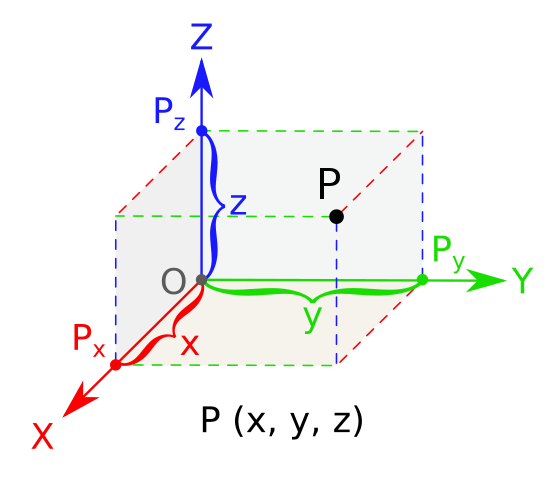
\includegraphics[scale=0.25]{images/1_Introduction/549px-Coord_planes_color.svg.png}
    \caption{Ο τρισδιάστατος χώρος, από το Wikipedia \url{https://en.wikipedia.org/wiki/Three-dimensional_space}}
\end{figure}

Τα διανύσματα μπορούν επίσης να προστεθούν, αφαιρεθούν και να πολλαπλασιάζονται μεταξύ τους. Παρακάτω θα αναλύσουμε τους κανόνες τις
διανυσματικής άλγεβρας.

Κατά την πρόσθεση, έστω για $\vec{A}$ και $\vec{B}$ το άθροισμα τους ορίζεται

\begin{equation}
    \vec{A} + \vec{B} = (A_x + B_x, A_y + B_y, A_z + B_z) = \vec{C} = (C_x, C_y, C_z)
\end{equation}

δηλαδή κάθε συνιστώστα τις διάστασης προστίθεται με τη συνιστώσα του άλλου διανύσματος στην ίδια διάσταση. Για παράδειγμα, έστω
$\vec{A} = (3, 2, -5)$ και $\vec{B} = (0, -2, \sqrt{2})$ τότε το άθροισμα τους είναι:

\begin{equation}
    \vec{A} + \vec{B} = (3+0,2-2,-5+\sqrt{2}) = \vec{C} = (3,0,-5+\sqrt{2})
\end{equation}

Πριν ορίσουμε τη διαίρεση θα ορίσουμε το αντίστροφο ενός διανύσματος. Ο αντίστροφος ενός διανύσματος $\vec{A} = (A_x, A_y, A_z)$
είναι:

\begin{equation}
    -\vec{A} = (-A_x, -A_y, -A_z)
\end{equation}

Εφόσον ορίσαμε τον αντίστροφο, η αφαίρεση ορίζεται εύκολα. Έστω $\vec{A}$ και $\vec{B}$ η διαφορά τους είναι:

\begin{equation}
    \vec{A} - \vec{B} = \vec{A} + (-\vec{B}) = (A_x - B_x, A_y - B_y, A_z - B_z) = \vec{C} = (C_x, C_y, C_z)
\end{equation}

Για παράδειγμα, έστω $\vec{A} = (3, 2, -5)$ και $\vec{B} = (0, -2, \sqrt{2})$ τότε η διαφορά τους είναι:

\begin{equation}
    \vec{A} - \vec{B} = \vec{A} + (-\vec{B}) = (3-0,2-(-2),-5-\sqrt{2}) = \vec{C} = (3,4,-5-\sqrt{2})
\end{equation}

Τέλος θα δείξουμε τον πολλαπλασιασμό διανυσμάτων. Για την ακρίβρεια, ο πολλαπλασιασμός διάνυσμα με διανύσμα ονομάζεται
βαθμωτό γινόμενο των διανυσμάτων - βαθμωτό γιατί η πράξη παράγει βαθμωτό μέγεθος και όχι διανυσματικό. Το βαθμωτό
γινόμενο δυο διανυσμάτων $\vec{A}$ και $\vec{B}$ ορίζεται:

\begin{equation}
    \vec{A} \cdot \vec{B} = A_x \cdot B_x + A_y \cdot B_y + A_z \cdot B_z = c, \text{όπου } c \text{ βαθμωτό μέγεθος}
\end{equation}

Για παράδειγμα, έστω τα διανύσματα $\vec{A} = (3, 2, 6)$ και $\vec{B} = (-1, 5, \frac{1}{2})$ τότε το βαθμωτό γινόμενο
ορίζεται ως εξής:

\begin{equation}
    \vec{A} \cdot \vec{B} = 3 \cdot -1 + 2 \cdot 5 + 6 \cdot \frac{1}{2} = -3 + 10 + 3 = 10
\end{equation}

θέλουμε να επισημάνουμε την προσοχή ότι στον τύπο 1.19 το απότελεσμα, $10$, είναι βαθμωτό. Μια ειδική περίπτωση του
βαθμωτού γινομένου είναι ο πολλαπλασιασμός ενός διανύσματος με ένα βαθμωτό μέγεθος, με ένα συντελεστή. Έστω ένα βαθμωτό
μέγεθος $r$ και ένα διάνυσμα $\vec{A}$ τότε το βαθμωτό γινόμενο τους είναι:

\begin{equation}
    r\vec{A}  = (rA_x, rA_y, rA_z)
\end{equation}

Πρέπει να προσέξουμε ότι το αποτέλεσμα είναι διανυσματικό μέγεθος αυτή τη φορά. Σαν γενικό κανόνα θα ορίσουμε:

\begin{enumerate}
    \item όταν θέλουμε το γινόμενο ανάμεσα σε διανύσματα, το αποτέλεσμα θα είναι πάντα βαθμωτό μέγεθος, και
    \item όταν θέλουμε το γινόμενο ανάμεσα σε ένα διάνυσμα και έναν βαθμωτό συντελεστή, το αποτέλεσμα θα είναι πάντα διανυσματικό μέγεθος
\end{enumerate}

\subsection{Ο συμβολισμός Dirac}
\subsection{Ο διανυσματικός χώρος Hilbert}
\subsection{Διανυσματικοί τελεστές και πινακοειδής αναπαράσταση τους}
\subsection{Το τανυστικό γινόμενο και τα σύνθετα κβαντικά συστήματα}
\subsection{Το qubit}
\subsection{Οι κβαντικές λογικές πύλες}

\section{Εισαγωγικά θέματα με το Qiskit και την Python}
\subsection{Διαχείριση λογισμικού με το Python 3 virtual enviroment και το pip}
\subsection{Κβαντικά κυκλώματα και καταχωρητές}
\subsection{Κλασικοί καταχωρητές και μετρήσεις}
